\section{DFA}
\label{sec:dfa}

\begin{figure}[h]
  \centering
  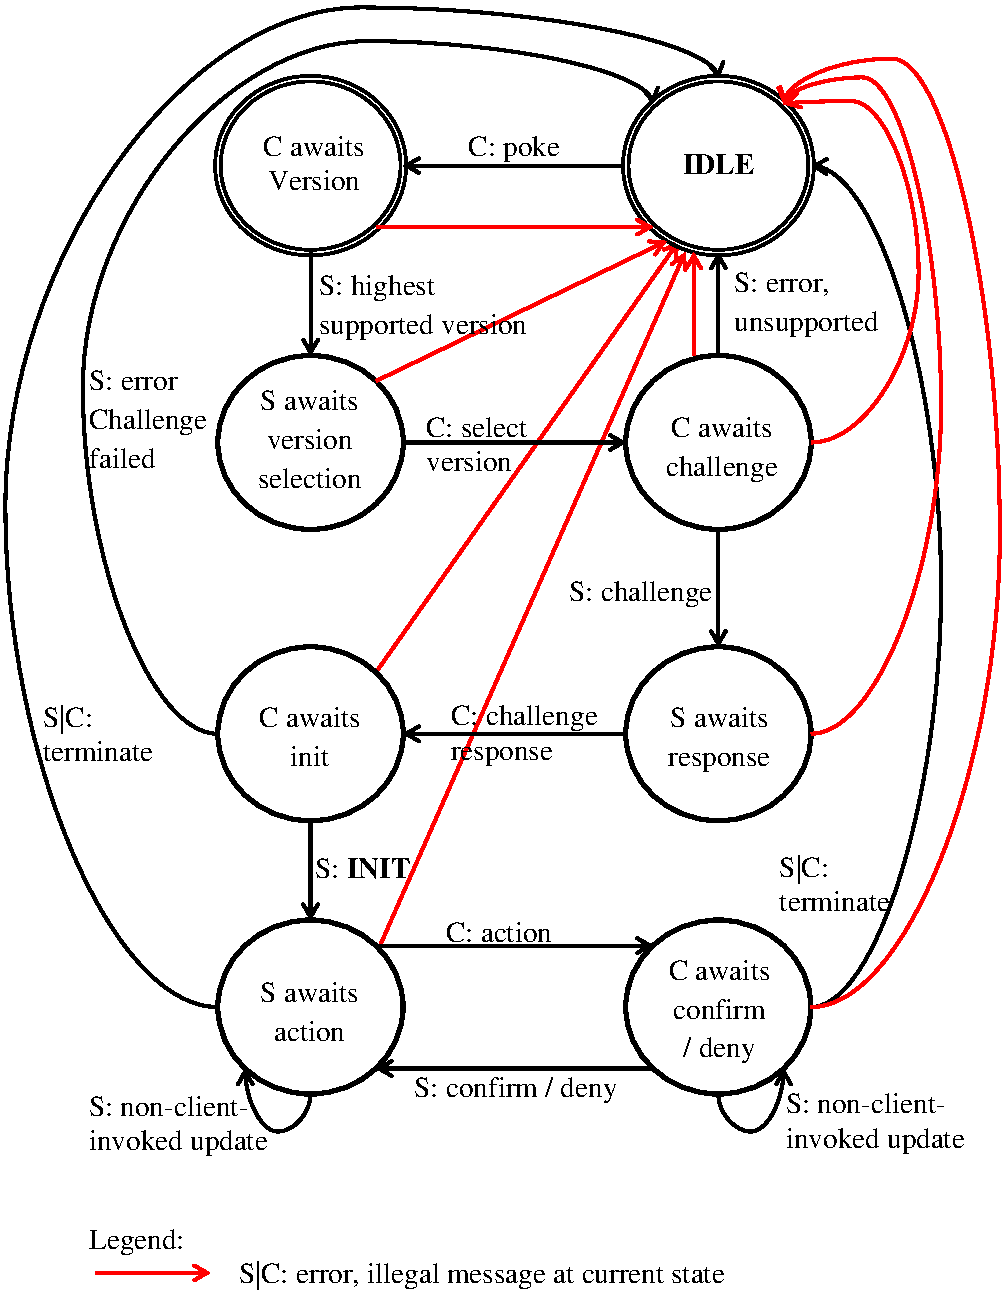
\includegraphics[width=4.95in]{figures/dfa.pdf}
  \caption{DFA illustration for the RSHC protocol.}
  \label{fig:dfa:dfa}
\end{figure}

An illustration of a DFA for RSHC is shown in \figr{fig:dfa:dfa}. Most of the states consist of handshake and initialization. After the main communication is in progress, there are only two states: the server awaits a client action (bottom left) and the client awaits a server confirmation / denial (bottom right). These two states illustrate the synchronous ``ping-pong'' communication between the server and the client. In addition, in both states the server may send the client a non-client-invoked action (every time the state of the house changed not due to this client's actions). Potential directions to extend the DFA (with new states or messages) are discussed in \sect{sec:extend}.

We chose to use only two states for the main communication phase of the protocol for simplicity. However, we can pair a DFA state to each subset of legal messages, which means a state for every configuration of the house: the states of all monitored devices. This approach would yield a number of states exponential in the number of devices, and a correspondence between the states of the protocol to the states of the application. Since the two-states model is sufficient for representation, it is chosen for the illustration of the protocol.
